%================================================================
\chapter{Bayesian Inference}\label{chap:bayesian}
%================================================================

\epigraph{A decision was wise, even though it led to disastrous consequences, if the evidence at hand indicated it was the best one to make; and a decision was foolish, even though it led to the happiest possible con-\\sequences, if it was unreasonable to expect those consequences.}{Herodotus, around 500 BC}


The aim of statistical inference is to learn about underlying properties of a population from observed data.  In statistical inference, there are, broadly speaking, two paradigms for the analysis of observed data: \textit{frequentist} inference and \textit{Bayesian} inference. These often differ with each other on the fundamental interpretation of probability. In the frequentist view, the probabilities of events are defined as their relative frequencies in a repeatable objective process, and are thus ideally devoid of opinion. From a Bayesian perspective, probabilities are measures that quantifies the uncertainty level of statements based on the degree of belief about the state of the world. Probabilities can be assigned to any statement, even when a random process is not involved. Bayesian inference is the process of revising beliefs about the state of the world in the light of new evidence.     

This chapter introduces the fundamentals of Bayesian inference, with a particular focus on parameter inference. The content of this chapter is mainly based on the material in the Bayesian textbooks \cite{BDA}, \cite{BAP} and \cite{Sivia}.


%================================================================
\section{Bayes' Theorem}\label{sec:bayes_paradigm}
%================================================================

In terms of parameter inference, the Bayesian approach differs from the frequentist in that unknown parameters $\theta$ are treated as random variables rather than fixed quantities. In the Bayesian paradigm, all available information about an unknown parameter is incorporated in a \textit{prior probability distribution}, expressing our beliefs before some evidence is taken into account. We usually have a prior pdf $\prior$, since there will typically be a continuum of possible values of a parameter rather than just a discrete set. In the case of substantial prior knowledge about a parameter $\theta$, the prior pdf is narrow and concentrated about some central value, whereas a lack of information yield a wider and relatively flat prior pdf as shown in \autoref{fig:prior_illustration}. The prior is often specified by a particular distribution among a set of well-known and tractable distributions, with the purpose of making evaluation of prior probabilities and random generation of $\theta$ values straightforward.

\begin{figure}[H]
    \centering
    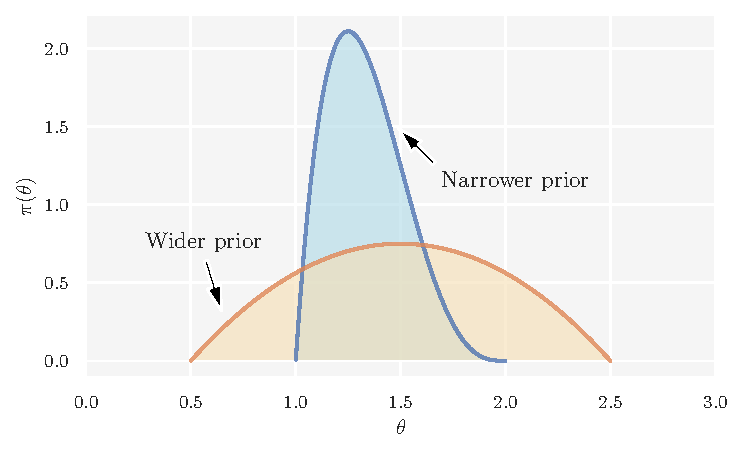
\includegraphics[scale=1.0]{prior_plot}
    \caption{Two prior distributions $\pi (\theta)$. A narrow concentrated prior (more certainty) about some central value and a wider less informative prior (less certainty).}
    \label{fig:prior_illustration}
    %\source{Figure 14.3 in \cite{STK}.}
\end{figure}

Our prior state of knowledge is modified by data $y$, obtained by performing experiments, through the conditional \textit{sampling distribution} $\lhood$. When regarded as a function of $\theta$, for fixed $y$, $\lhood$ is called the \textit{likelihood function}. In order to make probability statements about $\theta$ given sample data $y$, a probabilistic model representing the joint probability distribution for $\theta$ and $y$ must be provided. The joint pmf or pdf can be written as a product of the prior distribution $\prior$ and the likelihood function $\lhood$:

\begin{equation*}
    \joint = \lhood \prior .
\end{equation*}

At this point, Bayes' theorem is used to produce the \textit{posterior distribution}, which represents our state of knowledge about $\theta$ in the light of $y$. A common incarnation of Bayes' theorem is:

\begin{equation}\label{eq:bayes_theorem}
    \posterior = \frac{\joint}{p(y)}  = \frac{\lhood \prior}{p(y)},
\end{equation}

where the marginal probability of the data $p(y) = \int \lhood \prior \dd \theta$ in the case of continuous parameters, or, in the case of a discrete set of parameters, $p(y) = \sum_\theta \lhood \prior$, where the sum is over all possible values of $\theta$.

$p(y)$ is the same for all possible $\theta$, as it does not depend on $\theta$. With fixed $y$, this factor can thus be omitted in parameter inference since it constitutes a normalizing constant and does not enter into determining the relative posterior probabilities of different values of $\theta$. Omitting the factor $p(y)$ yields the unnormalized posterior distribution: 

\begin{equation}\label{eq:bayes_unnorm}
    \posterior \propto p(\theta, y) =  \lhood \prior .
\end{equation}

In this formulation, $\lhood$ is taken as a function of $\theta$ and not $y$.  

The core of Bayesian inference is encapsulated in \autoref{eq:bayes_theorem} and \autoref{eq:bayes_unnorm}. The principal task is to develop the joint probability model $\joint$ and perform the computations to obtain the posterior $\posterior$.


%================================================================
\section{Prior and Posterior Predictive Distributions}\label{sec:predictive_dist}
%\section{Prior and Posterior Predictive Distributions}\label{sec:predictive}
%\section{Single-parameter Models}\label{sec:single_inference}
%================================================================  

Before observing any data $y$, we simply have the chosen model, i.e., the likelihood, $\lhood$, and the prior distribution of $\theta$, $\prior$. To make predictive inference about the expected future data, $\hat{y}$, encoded in the prior assumptions, we calculate the marginal distribution of $y$, that is, the distribution of $y \mid \theta$ averaged over all possible values of $\theta$:

\begin{equation}\label{eq:prior_pred}
    p \qty(\hat{y}) = \int \lhood \prior \dd{\theta}.
\end{equation}

\autoref{eq:prior_pred} is called the \textit{prior predictive distribution}. 

Once we have a posterior, it is possible to generate predictions $\hat{y}$ following a similar logic. The \textit{posterior predictive distribution} is calculated by marginalizing the distribution of $\hat{y} \mid \theta$ over the posterior distribution: 

\begin{equation}\label{eq:post_pred}
    p \qty( \hat{y} \mid y ) =\int p \qty(\hat{y} \mid \theta) \posterior \dd{\theta}.
\end{equation} 

Thus, the posterior predictive distribution is an average of conditional predictions over the posterior distribution of $\theta$.


%================================================================
\section{Parameter Inference}\label{sec:param_inference}
%================================================================  

The way in which Bayes' theorem operates is best seen through examples. In the following we discuss Bayesian inference in the context of a statistical model where the closed form is available. %Such models are sometimes unrealistic, but their analysis often provides a useful starting point when it comes to constructing more realistic models.  

%================================================================
\subsection{The Beta-Binomial Model and the Effect of Priors}\label{sec:coin_flipping}
%===============================================================

The beta-binomial model is one of the simplest Bayesian models, and useful for introducing important concepts and computational methods in Bayesian analysis. The model is often illustrated in the context of the classical coin-flipping problem, where only a single scalar parameter, the success probability $\theta$, is to be estimated. 

In the coin-flipping problem, we toss a coin $n$ times and record the observations: either \textit{heads} or \textit{tails}. Based on this data, we try to answer questions such as \textit{is the coin fair?} Or, more generally, \textit{how biased is the coin?} In order to estimate the bias of a coin in a Bayesian setting, we need observed data, a probabilistic model of the data generating process, i.e., the likelihood, and a prior placed on the unknown model parameter. For this example, we assume that the data-gathering part is already done and we have recorded the number of heads after a number of coin flips. The bias of the coin is represented by the $\theta$ parameter, and we say that a coin with $\theta=1$ will always land heads, one with $\theta=0$ always tails and one with $\theta=0.5$ has an equal chance of landing either heads or tails. Assuming that only two outcomes are possible, heads or tails, and the random variable \textit{coin toss} is independent and identically distributed (iid), a candidate for the likelihood is the binomial distribution: 

\begin{equation}\label{eq:coin_flip_likelihood}
    \lhood = \binom{n}{y} \theta^y \qty(1 - \theta)^{n-y}.
\end{equation}

This is a discrete distribution returning the probability of getting $y$ heads (or in general, successes) out of $n$ coin tosses (or in general, trials or experiments) given a fixed value of $\theta$ (probability of success). 

\autoref{fig:binom_distribution} illustrates the binomial distribution for different $\theta$. From the figure we see that $\theta$ indicates how likely it is to obtain a head when tossing a coin, making the binomial distribution a reasonable choice for the likelihood. 

\begin{figure}[ht]
    \centering
    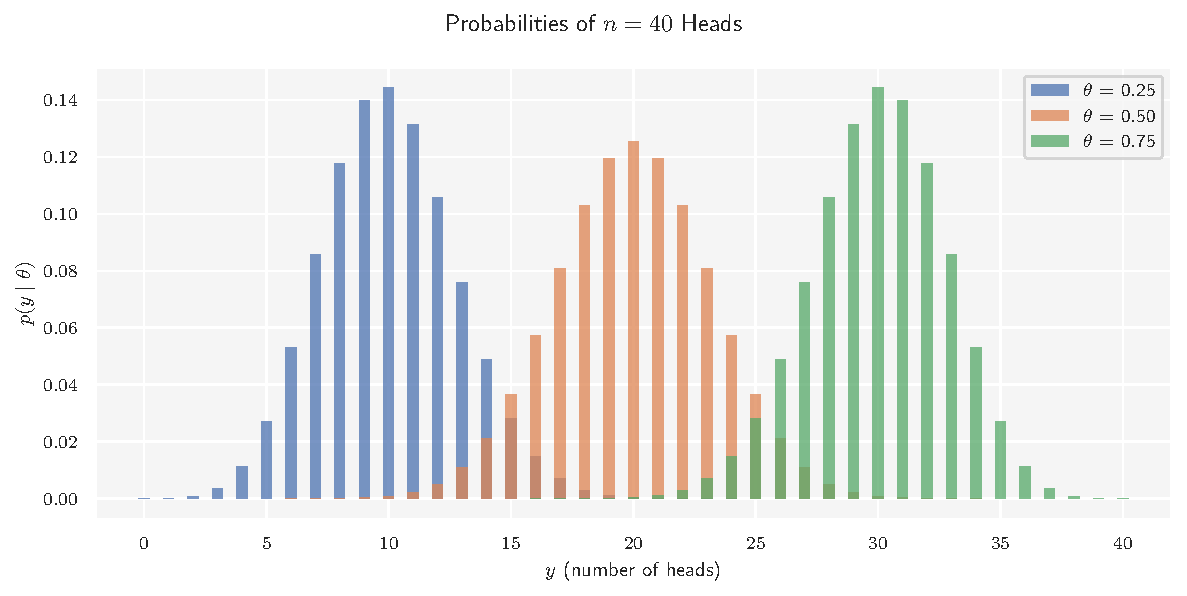
\includegraphics[scale=1]{binomial_distribution}
    \caption{Binomial distributions with $n=40$ coin flips and different success probabilities $\theta$. The coin is biased towards tails when $\theta < 0.5$ (blue) and heads when $\theta > 0.5$ (green). For $\theta=0.5$ (orange) the coin is unbiased (or fair). The legend indicates the values of the $\theta$.}
    \label{fig:binom_distribution}
\end{figure} 

If the value of $\theta$ is known, the binomial distribution tells us the expected distribution of heads. However, $\theta$ is an unknown model parameter, and thus we need to place a prior on it. For mathematical convenience, we choose a family of prior densities that lead to simple posterior densities. Considered as a function of $\theta$, \autoref{eq:coin_flip_likelihood} is of the form: 

\begin{equation*}
    \lhood \propto \theta^a \qty(1 - \theta)^b.
\end{equation*} 

If the prior density is of the same form, with its own parameterization of $a$ and $b$, then the posterior will also be of this form. Such a prior density can be parameterized as: 

\begin{equation*}
    \prior \propto \theta^{\alpha - 1} \qty(1 - \theta)^{\beta -1},
\end{equation*}

which is the beta distribution with shape parameters $\alpha>0$ and $\beta>0$. The parameters of the prior distribution are often called \textit{hyperparameters}. In order to ensure that the total probability is 1, the beta function,

\begin{equation*}
    B (\alpha, \beta) = \frac{\Gamma(\alpha)\Gamma(\beta)}{\Gamma(\alpha + \beta)},
\end{equation*}

where $\Gamma (z)$ is the gamma function, can be used as a normalizing constant:

\begin{equation}\label{eq:beta_prior}
    \prior = \frac{1}{B(\alpha, \beta)} \theta^{\alpha -1} (1-\theta)^{\beta -1}.
\end{equation}

The beta distribution is defined on the interval $[0, 1]$. \autoref{fig:beta_distribution} shows the beta distribution with different shape parameters. The figure displays the versatility of the beta distribution; the distribution adopts several shapes, determined by the shape parameters, including the uniform distribution with $\alpha = \beta = 1$. The uniform (blue) prior represents all the possible values for $\theta$ being equally likely a priori. The Gaussian-like (orange) prior is concentrated about $\theta=0.5$, and reflects a belief that the coin is equally probable to land heads or tails. The reverse J-shaped (green) prior is skewed towards a tail-biased outcome.

\begin{figure}[ht]
    \centering
    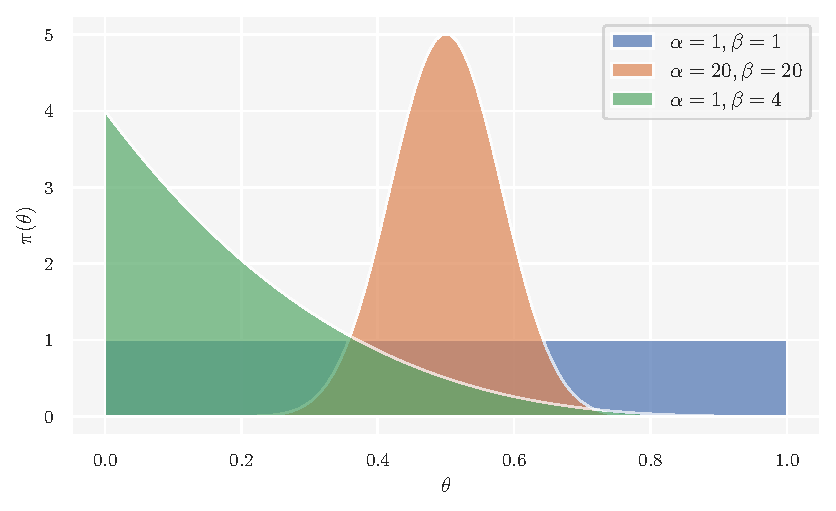
\includegraphics[scale=1]{beta_distribution}
    \caption{The beta prior probability distribution with different parameterizations by the two positive shape parameters. The beta distribution adopts several shapes controlled by the shape parameters; $\alpha=\beta=1$ gives a uniform distribution (blue), $\alpha=\beta=20$ gives a bell curve centered at $\theta=0.5$ (orange) and finally $\alpha=1$ and $\beta=2$ gives a reverse J-shaped distribution with a right tail (green).
    }
    \label{fig:beta_distribution}
\end{figure} 


Bayes' theorem, \autoref{eq:bayes_unnorm}, states that the posterior is proportional to the product of the likelihood and the prior. Thus, for our problem the posterior density for $\theta$ is given as: 

\begin{equation*}
    \pi (\theta \mid y) \propto \binom{n}{y} \theta^y (1-\theta)^{n-y} \frac{1}{B(\alpha, \beta)} \theta^{\alpha-1}(1-\theta)^{\beta -1}.
\end{equation*}

With fixed $n$ and $y$, the factor $\binom{n}{y}$ does not depend on the unknown parameter $\theta$, and neither does the beta function $B(\alpha, \beta)$. Thus can both be treated as constants when calculating the posterior distribution of $\theta$:

\begin{align*}
    \posterior &\propto \theta^y (1-\theta)^{n-y} \theta^{\alpha-1}(1-\theta)^{\beta -1} \\
    &= \theta^{\alpha + y -1} (1-\theta)^{\beta + n-y -1},
\end{align*}

or, more concisely:

\begin{equation}\label{eq:coin_posterior}
    \posterior \propto \theta^{\alpha' -1} (1-\theta)^{\beta' -1},
\end{equation}

with $\alpha'=\alpha+y$ and $\beta' = \beta + n - y$. We recognize that the expression above has the same functional form as the unnormalized beta distribution. The property that the posterior distribution follows the same parametric form as the prior distribution is called \textit{conjugacy}, and we say that the beta distribution is a \textit{conjugate prior} for the binomial likelihood.  

\autoref{fig:coin_flip_posterior} shows how the posteriors for the priors in \autoref{fig:beta_distribution} evolve as more and more data become available. For easier comparison, they have all been scaled vertically to have the same maximum value. \autoref{fig:coin_flip_posterior} clearly reveals the effect of the different priors; when there are few data, the shape of the posteriors vary in detail; as the number of data increases, the shape and location of the posteriors tend to converge and they all become sharply peaked. Since the priors reflect the different information or assumptions before the results, and the posteriors the updated knowledge in the light of data, this seems quite reasonable. If the data only are the outcome of a few flips, the analysis of these data is dominated by the prior information. However, as the data increases, the posterior is dominated by the likelihood and we are eventually led to the same conclusions regardless of our initial beliefs. In the limit of infinite data, all priors will provide the same posterior. From a practical point of view, we could obtain nearly indistinguishable posteriors for a finite amount of data. Thus, the choice of the prior becomes largely irrelevant given a sufficiently large amount of data.

\begin{figure}[H]
    \centering
    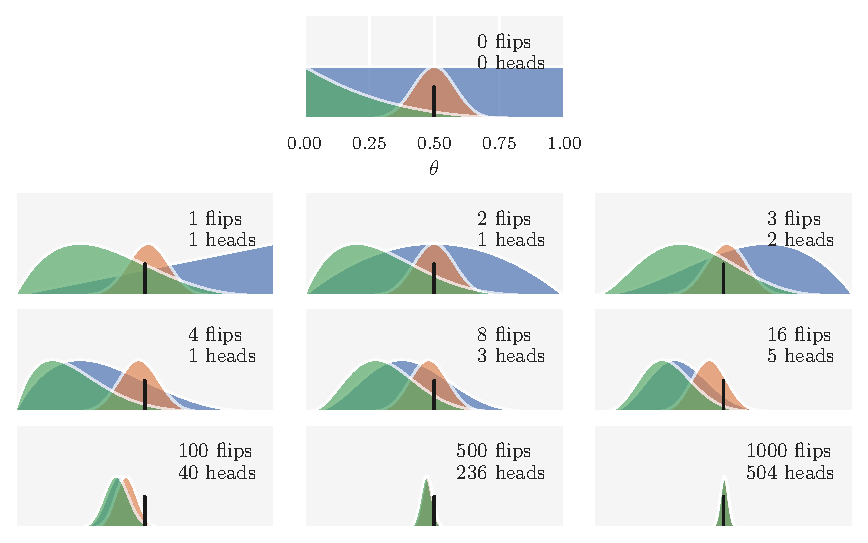
\includegraphics[scale=1]{coin_flip_posterior}
    \caption{The effect of different priors on the posterior as the number of data available increases. To aid in the comparison, they have all been scaled vertically to have the same maximum value. The number of data analyzed is indicated at the upper right-hand corner of each panel. In the first panel there are zero flips, and thus the densities represent the priors from \autoref{fig:beta_distribution}. The ground truth, $\theta=0.5$ (the coin is indeed fair), is indicated by the black vertical line. 
    }
    \label{fig:coin_flip_posterior}
\end{figure} 

Priors are often categorized by the information they incorporate about parameters as either \textit{noninformative}, \textit{weakly informative} or \textit{informative}. If the prior is noninformative, the posterior is data-driven, as illustrated by the uniform (blue) prior in \autoref{fig:coin_flip_posterior}. On the other hand, if the prior is informative, as illustrated by the bell curve (orange) prior in \autoref{fig:coin_flip_posterior}, the posterior is a mixture of the prior and the data. However, as mentioned and seen in the figure, the data will overwhelm the prior and dominate the posterior in the case of large amounts of data. Weakly informed priors are constructed to purposely include less information than we actually have. They can be useful if we want to let the data speak but not model complete ignorance.



%================================================================
\section{Bayesian Computation}
%================================================================

While conceptually simple, Bayesian analysis can be mathematically and numerically challenging. For a long time, Bayesians restricted their attention to conjugate families where posteriors can be computed analytically in closed form. However, realistic probabilistic models often lead to analytically intractable expressions. The arrival of the computational era and development of sampling-based numerical methods have transformed the Bayesian analysis practice. In this section we discuss estimating the posterior numerically using algorithms from the Markov Chain Monte Carlo (MCMC) family. 


%================================================================
\subsection{Markov Chain Monte Carlo}
%================================================================

There have been devised a suite of methods for constructing and sampling from arbitrary posterior distributions, but Markov chain Monte Carlo (MCMC) methods have become the predominant computational strategy for Bayesian inference. The term \textit{Monte Carlo} refers to methods that rely on the generation of random samples from a distribution of interest. In general, a \textit{Markov chain} is a sequence of states for which the probability of transitioning to the next state depends only on the present state. That the next state is only conditional on the present state and thus independent of the previous states is known as the Markov property. By providing a starting point, such a chain can perform a random walk between the states according to the transition probabilities. Hence, the main idea of MCMC is to draw samples of $\theta_t$ sequentially with the distribution of sampled draws depending on the previous sample $\theta_{t-1}$ to construct a Markov chain $\qty{\theta_t, t=0,1,2,...}$. The key to the method's success is finding a Markov chain with transitions proportional to the target posterior distribution, $\posterior$. In other words, the success is determined by whether the chain is able to improve the sampling distribution at each step in the simulations, in the sense of converging to the posterior distribution. 


%================================================================
\subsection{The Metropolis Algorithm}
%================================================================

The Metropolis algorithm is one of the most established MCMC sampling methods and was originally proposed in \cite{Metropolis}. It was later generalized by Hastings in \cite{Hastings} into the Metropolis-Hastings algorithm. In its original form, the Metropolis algorithm is an adaptation of a random walk that explores the local neighborhood of the current value of the Markov chain. It uses an acceptance/rejection rule to converge to the specified target distribution. The algorithm proceeds as follows:

\begin{enumerate}
    \item Initialize the Markov chain with a starting point $\theta_0$ for which $\pi \qty(\theta_0 \mid y)>0$. Conceptually, it makes most sense to draw $\theta_0$ from the prior $\pi(\theta)$, though it can be chosen by making an educated guess. 
    \item For each iteration of $t$, with $t=1, 2, ...$: 
    \begin{itemize}
        \item[(a)] Sample a \textit{proposal} parameter $\theta^*$ from the \textit{proposal distribution} (also called the \textit{jumping distribution}) $q \qty(\theta^* \mid \theta_{t-1})$ from which sampling is easily done. For the Metropolis algorithm (but not the Metropolis-Hastings algorithm), the proposal distribution must be symmetric, satisfying the condition $q \qty(\theta^* = \theta_a \mid \theta_{t-1} = \theta_b) = q \qty(\theta^* = \theta_b \mid \theta_{t-1} = \theta_a)$ for all $\theta_a$, $\theta_b$ and $t$. Both the normal and uniform distributions are examples of symmetric distributions that satisfies this condition. 
        \item[(b)] Evaluate the quality of the proposal $\theta^*$ by calculating the ratio of posterior densities: 
        \begin{equation}\label{eq:metropolis_ratio}
            r = \frac{\pi \qty(\theta^* \mid y)}{\pi \qty(\theta_{t-1} \mid y)} = \frac{p \qty(y \mid \theta^*) \pi \qty(\theta^*)}{p \qty(y \mid \theta_{t-1}) \pi \qty(\theta_{t-1})}.
        \end{equation} 
        Note that we do not actually use the posterior directly, but rather the proportionality given by Bayes' theorem (\autoref{eq:bayes_unnorm}). If the posterior density of $\theta^*$ is greater than that of $\theta_{t-1}$, the ratio of the posterior densities will be greater than 1 and we will accept the proposal as the next state of the chain. If the posterior density is greater for $\theta_{t-1}$, we will not necessarily discard the proposal $\theta^*$. Less probable parameter values are accepted probabilistically:
        \item[(c)] Calculate the Metropolis acceptance criterion:
        \begin{equation}\label{eq:metropolis_acceptance}
            \alpha = \min \qty(1, r),
        \end{equation}
        and set
        \begin{equation*}
            \theta_t = \begin{cases}
            \theta^* &\qquad \text{with probability } \alpha 
            \\
            \theta_{t-1} &\qquad \text{with probability } 1 - \alpha 
            \end{cases}.
        \end{equation*}
        In this way, the Metropolis algorithm ensures that the chain tends to move towards the highest density regions of the posterior, but it can still move away from these high-density regions and towards the tails of the posterior. The chain being able to assume all possible states, given enough time, is called \textit{ergodicity}, and is an important feature of the Metropolis algorithm. 
    \end{itemize}
\end{enumerate}

To implement the algorithm in a computer program, step (c) requires, after computing $\alpha$ for $\theta^*$, the generation of a uniform random number $u \sim \mathrm{U}(0,1)$. If $u \leq \alpha$, we accept the proposal and set $\theta_t = \theta^*$. If $u > \alpha$, we reject the proposal and set $\theta_t = \theta_{t-1}$ instead. Note that when the proposal is not accepted, this still counts as an iteration of the algorithm. 

The normal distribution, $\mathrm{N}\qty(\mu, \sigma^2)$, is an example of a symmetric proposal distribution. Conditioning the normal distribution on the previous value $\theta_{t-1}$ of the chain means that the location parameter $\mu=\theta_{t-1}$. The scale parameter $\sigma$ is a tuning parameter that we increase or decrease if the acceptance rate of the simulations is too high or low, respectively. According to \cite{BDA}, the optimal acceptance rate is 0.44 for single parameter inference problems and 0.23 for for inference problems concerning several parameters. 

\cref{alg:metropolis} summarizes the Metropolis algorithm.  

\begin{algorithm}[H]
\caption{Metropolis sampling}
\label{alg:metropolis}
\SetAlgoLined
\DontPrintSemicolon
 % Algorithm 
 \textbf{Inputs\,:}\;
 \vspace{-5mm}
 \begin{itemize}
     \item A target posterior density $\posterior \propto \lhood \prior$ consisting of a prior $\prior$ and likelihood $\lhood$. 
     \item A symmetric Markov proposal density $q \qty(\theta^* \mid \theta)$.
     \item An integer $N>0$.
 \end{itemize}
 
 \vspace{5mm}
 \textbf{Initialize\,:}\;
 Sample $\theta_0 \sim \prior$.\;

 \vspace{5mm}
 \textbf{Sampling\,:}\;
 \For{$t=1, ..., N$}{ 
 Generate proposal $\theta^* \sim q \qty(\theta^* \mid \theta_{t-1})$. \; 
 Calculate acceptance criterion $\alpha = \min \qty(1, \dfrac{p \qty(y \mid \theta^*) \pi \qty(\theta^*)}{p \qty(y \mid \theta_{t-1}) \pi \qty(\theta_{t-1})})$. \;
 Sample $u \sim \mathrm{U}(0,1)$. \; 
 \vspace{2mm}
 \eIf{$u \leq \alpha$}{
   $\theta_t = \theta^*$\;
   }{
   $\theta_t = \theta_{t-1}$\;
  }
 }
\end{algorithm}



%================================================================
\section{Density Estimation}
%================================================================ 

The probability density function (pdf) is a fundamental concept in statistics. When we estimate the posterior numerically, we obtain random samples of $\theta$ drawn from the posterior density $\posterior$ but not the posterior pdf itself. In this section, we briefly discuss \textit{density estimation}, that is, methods for constructing an estimate of the pdf from sample data. The focus will be on \textit{nonparametric} approaches to density estimation. The content of this section is based on the material in the statistical learning textbooks \cite{ESL} and \cite{Bishop}.

\subsection{Histograms} 


--- 

Standard histograms simply partition $x$ into distinct bins of width $\Delta_i$ and then count the number $n_i$ observations of $x$ falling in bin $i$. In order to turn this count into a normalized probability density we simply divide by the total number $N$ of observations and by the width $\Delta_i$ of the bins to obtain probability values for each bin given by 

$$ p_i = \frac{n_i}{N \Delta_i}$$ 

for which it is easily seen that $\int p(x) dx = 1$. This gives a model for the density $p(x)$ that is constant over the width of each bin, and often the bins are chosen to have the same width $\Delta_i = \Delta$.


---

rules-of-thumb like Scott’s rule and the Freedman-Diaconis rule are fast and convenient, but their strong assumptions about the data might make them less ideal for complicated distributions. 

---

The most basic density estimator is the histogram [1]. A histogram is an approximate representation of data that divides the data into discrete bins and counts the number of points that fall in each bin. In a more general mathematical sense, a histogram is defined as follows [1]. We denote the density estimator by $\hat{f}$ and assume we are given a sample of $n$ observations $X_1, ..., X_n$ whose underlying density is to be estimated. Given an origin $x_0$ and a bin width $h$, the bins of the histogram are defined as the intervals $[x_0 + mh, x_0 + (m+1)h)$ for $m$ positive and negative integers. The histogram is then defined by

\begin{equation*}
    \hat{f}(x) = \frac{1}{nh} \times (\text{no. of } X_i \text{ in the same bin as } x)
\end{equation*}

The histogram can be generalized by allowing the bin widths to vary. Then the estimate becomes 

\begin{equation*}
    \hat{f}(x) = \frac{1}{n} \times \frac{(\text{no. of } X_i \text{ in the same bin as } x)}{\text{width of bin containing }x}
\end{equation*}


---


\subsubsection*{Original papers:} 

Scott, D. (1979). On optimal and data-based histograms \url{http://biomet.oxfordjournals.org/content/66/3/605}

Freedman, D. and Diaconis, P. (1981). On the histogram as a density estimator: L2 theory \url{http://www.springerlink.com/content/mp364022824748n3/}

\textbf{See also SNL thesis:} Primer on density estimation (parametric/non-parametric) and includes neural density estimators. 


non-parametric way to estimate the probability density function of a random variable

\subsection{Kernel Density Estimation}

Histograms have been a popular visualization option since at least the 18th century, in part because they are easily generated by hand. More recently, as extensive computing power has become available in everyday devices such as laptops and cell phones, we see them increasingly being replaced by density plots. In a density plot, we attempt to visualize the underlying probability distribution of the data by drawing an appropriate continuous curve (Figure 7.3). This curve needs to be estimated from the data, and the most commonly used method for this estimation procedure is called kernel density estimation. In kernel density estimation, we draw a continuous curve (the kernel) with a small width (controlled by a parameter called bandwidth) at the location of each data point, and then we add up all these curves to obtain the final density estimate

Analogous to the binwidth of a histogram, a density plot has a parameter called the bandwidth that changes the individual kernels and significantly affects the final result of the plot. The plotting library will choose a reasonable value of the bandwidth for us (by default using the ‘scott’ estimate)

With many data points the rug plot can become overcrowded, but for some datasets, it can be helpful to view every data point. The rug plot also lets us see how the density plot “creates” data where none exists because it makes a kernel distribution at each data point. These distributions can leak over the range of the original data and give the impression that Alaska Airlines has delays that are both shorter and longer than actually recorded. We need to be careful about this artifact of density plots and point it out to viewers!

%================================================================
%\section{Gaussian Models and Posterior Checks}\label{sec:gaussian_models}
\section{Summarizing the Posterior}
%\section{Summarizing the Posterior}
%================================================================ 

The result of a Bayesian analysis is a posterior distribution which contains all the current information about the parameters $\theta$. The focus of this section will be on how we can summarize the obtained posteriors with graphical checks and numerical measures.

---

In this section, we will look at both numerical and graphical ways to summarize the posterior:

See Performance Metrics in introduction !!!!!


\subsection{Posterior Plot}

In principle, the posterior distribution contains all the information about the possible parameter values. In practice, we must also present the posterior distribution somehow. If the examined parameter $\theta$
  is one- or two dimensional, we can simply plot the posterior distribution. Or when we use simulation to obtain values from the posterior, we can draw a histogram or scatterplot of the simulated values from the posterior distribution. If the parameter vector has more than two dimensions, we can plot the marginal posterior distributions of the parameters of interest.
  
 However, we often also want to summarize the posterior distribution numerically. The usual summary statistics, such as the mean, median, mode, variance, standard devation and different quantiles, that are used to summarize probability distributions, can be used. These summary statistics are often also easier to present and interpret than the full posterior distribution.

\subsection{Point estimates}

People often choose the median, just because it is more robust to outliers than the mean, or use the mean just because is a simple and familiar concept, or because they think their observable is truly the average of some process at some level, like molecules bouncing to each other or genes interacting with themselves and the environment.

Commonly used summaries of location are the mean, median and mode(s) of the distribution; variation is commonly summarized by the standard deviation, the interquartile range and other quantiles. Each summary has its own interpretation: for example, the mean is the posterior expectation of the parameter, and the mode may be interpreted as the single 'most likely' value, given the data (and the model).

\url{https://en.wikipedia.org/wiki/Maximum_a_posteriori_estimation}

\url{http://bebi103.caltech.edu.s3-website-us-east-1.amazonaws.com/2015/tutorials/l06_credible_regions.html}

\url{https://bookdown.org/mrwhalen/bayes_book/summarizing-posterior-distributions.html}

\url{https://vasishth.github.io/bayescogsci/book/sec-priorpred.html}

\url{https://vioshyvo.github.io/Bayesian_inference/summarizing-the-posterior-distribution.html}

\subsection{Posterior quantiles and intervals}




THIS IS NEW

The result of a Bayesian analysis is a posterior distribution, and all the information about the parameters given a dataset and a model is contained in the posterior distribution. Thus, by summarizing the posterior, we are summarizing the logical consequences of a model and data. A common practice is to report, for each parameter, the mean (or mode or median) to have an idea of the location of the distribution and some measure, such as the standard deviation, to have an idea of the dispersion and hence the uncertainty in our estimate. The standard deviation works well for normal-like distributions but can be misleading for other type of distributions, such as skewed ones. So, an alternative is to use the following measure.

\subsection{Posterior Predictive Check}

The generated predictions $\hat{y}$ from the posterior predictive distribution, \autoref{eq:post_pred}, can be used to validate and criticize the model by comparing them with the observed data $y$. This is known as \textit{posterior predictive checks}. 

The main goal is to check for auto-consistency. The generated data and the observed data should look more or less similar, otherwise there was some problem during the modelling or some problem feeding the data to the model. But even in the absence of mistakes, differences could arise. Trying to understand the mistakes could lead us to improve models or at least to understand their limitations.  

---

To make inferences about an unknown variable, often called predictive inferences, we follow a similar logic. Before the data $y$ are considered, the distribution of unknown but observable $y$ is 

\begin{equation}\label{eq:prior_predictive}
    \pi (y) = \int \lhood \prior \dd{\theta}
\end{equation}

%BDA, side 7

Posterior predictive check
Comparing the data to the posterior predictions of the model is called a posterior predictive check. When there appear to be systematic discrepancies that would be meaningful to address, you should consider expanding or changing the model so it may be a better description of the data.

One way to evaluate whether the least unbelievable parameter values are any good is via a posterior predictive check. A posterior predictive check is an inspection of patterns in simulated data that are generated by typical posterior parameters values. The idea of a posterior predictive check is as follows: If the posterior parameter values really are good descriptions of the data, then the predicted data from the model should actually “look like” real data. If the patterns in the predicted data do not mirror the patterns in the actual data, then we are motivated to invent models that can produce the patterns of interest.

---

Posterior Predictive Distributions
For evaluating the fit of a model, perhaps the most flexible approach is to examine the Bayesian posterior predictive distribution. The posterior predictive distribution is the distribution of future observable data, based on the posterior distribution. It is defined as: 

eq same as 6.1 in BDA 

In this equation, $y_{rep}$ is future data that could be drawn from the posterior distribution, $y$ is the current data, and $\theta$ is the model parameter. Notice that the last two terms (prior to $d\theta$) are the posterior density for the parameter. The first term is the sampling density for future data, conditional on the parameter. This equation simply specifies a form for the distribution of future data, given the model parameter and data. If a model fits the current data well, then we expect that simulated future data should look much like the current data. Thus, we can simulate data from the posterior predictive distribution, compare it to the observed data, and determine whether the model has an appropriate fit. 

---

Following the same logic, prior predictive distribution  


\subsection{Measures of Predictive Accuracy}

Goodness of fit in Bayesian analyses is routinely assessed using a method referred to as the ‘Bayesian p-value’ and posterior predictive checks (Gelman et al., 1996).

s. 166/167 i BDA 


Fourth, when applying SNPE (or any other model-identification approach), validation of the results is of crucial importance, both to assess the accuracy of the inference procedure, as well as to identify possible limitations of the mechanistic model itself. In the example applications, we used several procedures for assessing the quality of the inferred posteriors. One common ingredient of these approaches is to sample from the inferred model, and search for systematic differences between observed and simulated data, e.g. to perform posterior predictive checks (Cook et al., 2006; Talts et al., 2018; Liepe et al., 2014; Lueckmann et al., 2017; Greenberg et al., 2019; Figure 2g, Figure 3f,g, Figure 4c, and Figure 5d). These approaches allow one to detect ‘failures’ of SNPE, that is, cases in which samples from the posterior do not reproduce the data. However, when diagnosing any Bayesian inference approach, it is challenging to rigorously rule out the possibility that additional parameter-settings (e.g. in an isolated ‘island’) would also explain the data. Thus, it is good practice to use multiple initializations of SNPE, and/or a large number of simulations in the initial round. There are challenges and opportunities ahead in further scaling and automating simulation-based inference approaches. However, in its current form, SNPE will be a powerful tool for quantitatively evaluating mechanistic hypotheses on neural data, and for designing better models of neural dynamics.

%================================================================
%\section{Gaussian Models and Posterior Checks}\label{sec:gaussian_models}
\subsection{Bayesian Analysis}
%\section{Summarizing the Posterior}
%================================================================


Posterior - all information

We will use a Gaussian model with unknown mean and variance to illustrate the following, since it is continuous and

The Bayesian Toolkit

One point that must be clear from the beginning is that the Bayesian approach is a complete inferential approach. Therefore, it covers confidence evaluation, testing, prediction, model checking, and point estimation. We will progres- sively cover the different facets of Bayesian analysis in other chapters of this book, but we address here the issue of confidence intervals because it is rather a straightforward step from point estimation.

normal models important blabla

As we saw in the previous section, conjugacy ensures tractable posteriors. Sufficent summary statistics, (mean and variance for normal)

The derivation requires some tedious algebra, so we simply state the result (Murphy, 07)

\url{https://en.wikipedia.org/wiki/Conjugate_prior#When_likelihood_function_is_a_continuous_distribution}


The comprehensive derivation can be found in appendix B. 

Devore, p. 781 

Note that the posterior mean $\mu_0'$ is a weighted average of the prior mean $\mu_0$ and the data mean $\bar{x}$, with weights that are the reciprocals of the prior variance and the variance of $\bar{x}$. It makes sense to define the \textbf{precision} as the reciprocal of the variance because a lower variance implies a more precise measurement and the weights then are the corresponding precisions. Furthermore, the posterior variance is the reciprocal of the sum of the reciprocals of the two variances, but this can be described much more simply by saying that the posterior precision is the sum of the prior precision plus the precision of $\bar{x}$.  


Sufficient statistics are useful in algebraic manipulations of likelihoods and posterior distributions.

sufficient summary statistics, lfi for cogsci, side 16, Fisher-Neyman Factorization Theorem

\url{https://bookdown.org/mrwhalen/bayes_book/summarizing-posterior-distributions.html}

Summarizing Posterior Distributions
Obtaining a posterior distribution is great, but does not provide us with much concrete to discuss or convey to others. Therefore, we need ways to distill the distribution into point estimates, or summary statistics. The most common summary statistics for posterior distributions will be the posterior mean, posterior mode and posterior median.

At times, there will be different reasons to use each summary statistic, but most often a safe assumption is to report the posterior mean $\pm$ posterior standard devition.

From a decision theory standpoint there technically are mathematical ways to determine which point estimate is the best to use in certian instances, but that is beyond the scope of this tutorial. However, here are the answers that come from magic (maybe I will post the proofs in the appendix:

1. If the loss function is quadratic, the best estimate is the posterior mean.
2. If the loss function is an absolute loss, the best estimate is the posterior median.
3. If the loss function is an All-or-nothing loss, the best estimate is the posterior mode

The posterior mode is just the expected value of the parameter estimate, using the posterior distribution.

Recall that a mode is simply the most frequent point in a data set. In a Bayesian distribution, this refers to the peak of the distribution (the parameterestimate with the highest overall weight). 

The posterior median refers to the value which divides the distribution in half. This is a bit more challenging to calculate by hand (and is the least frequently used summary statistic) but it is worth seeing where this value comes from.

We need to find the value $\theta$ which has 50\% of the probability to the left and 50\% to the right. It is also worth noting that the median is tricky to calculate for discrete distributions (hence why it is rarely seen).


Credible Intervals

There is a lot to say about the difference between Bayesian Credible Intervals and Classical Confidence Intervals. I will avoid this entire discourse and just say that in Bayesian statistics a Credible Interval is the interval in which we have a 95\% probabilistic belief the parameter is in that interval.

In Chapter 1, Thinking Probabilistically, we introduced the concept of posterior predictive checks, and, in subsequent chapters, we have used it as a way to evaluate how well models explain the same data that's used to fit the model. The purpose of posterior predictive checks is not to dictate that a model is wrong; we already know that! By performing posterior predictive checks, we hope to get a better grasp of the limitations of a model, either to properly acknowledge them, or to attempt to improve the model. Implicit, in the previous statement is the fact that models will not generally reproduce all aspects of a problem equally well. This is not generally a problem given that models are built with a purpose in mind. A posterior predictive check is a way to evaluate a model in the context of that purpose; thus, if we have more than one model, we can use posterior predictive checks to compare them.

%================================================================
%\section{Summarizing the Posterior}
%================================================================

In Bayesian inference, posterior beliefs about parameters are updated according to \textit{Bayes' theorem} upon observing data.  

The mean of this posterior distribution gives a point estimate of $\theta$. 

An interval having a posterior probability $.95$ gives a $95\%$ \textit{credibility} interval, an interval within which an unobserved parameter value falls with a particular probability, the Bayesian analogue of a $95\%$ confidence interval \cite[p. 777]{STK}.

Credible intervals 

HDI 

Energy

- mean, median, mode: point estimates

- variance and standard deviation: spread -> uncertainty 

- credible intervals, highest density posterior (hdp) 


RMSE, true value, SEM 

In practice, we generally do not have the value of the true parameter $\theta$ at hand. Instead, we have an estimation in the form of a posterior distribution. Thus, what we can do is find out the value of $\hat{\theta}$ that minimizes the expected loss function. By expected loss function, we mean the loss function averaged over the whole posterior distribution. 








%================================================================
%\section{Why Bayes?}
%================================================================

%End chapter with this? No, move to introduction
